\begin{center}
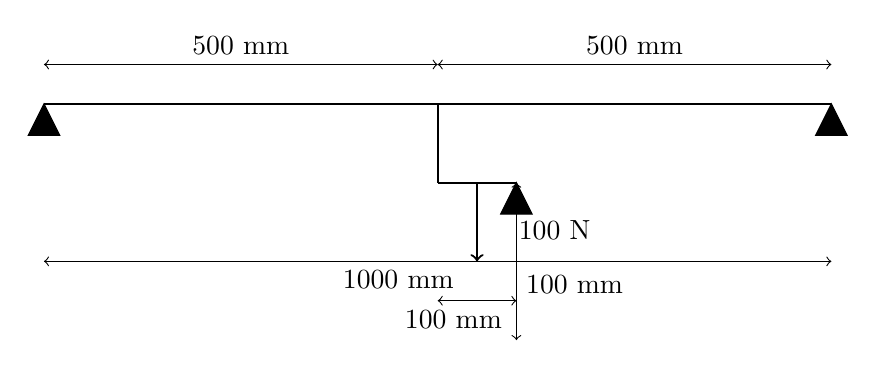
\begin{tikzpicture}
    % Beam horizontal section
    \draw[thick] (0,0) -- (10,0); % 1000 mm long beam
    
    % Beam step-down section
    \draw[thick] (5,0) -- (5,-1); % Vertical step-down 100 mm
    \draw[thick] (5,-1) -- (6,-1); % Horizontal part 100 mm
    
    % Force vector
    \draw[thick, ->] (5.5,-1) -- (5.5,-2) node[midway,right, yshift=-0.1cm, xshift= 0.4cm] {100 N}; % Downward force arrow
    
    % Supports
    \filldraw (0,0) -- (-0.2,-0.4) -- (0.2,-0.4) -- cycle; % Left triangle support
    \filldraw (10,0) -- (9.8,-0.4) -- (10.2,-0.4) -- cycle; % Right triangle support
    \filldraw (6,-1) -- (5.8,-1.4) -- (6.2,-1.4) -- cycle; % Middle triangle support at step
    
    % Dimension lines
    % Full length
    \draw[<->] (0,-2) -- (10,-2) node[midway, below, xshift=-0.5cm] {1000 mm}; 
    
    % Left section length
    \draw[<->] (0,0.5) -- (5,0.5) node[midway, above] {500 mm}; 
    
    % Right section length
    \draw[<->] (5,0.5) -- (10,0.5) node[midway, above] {500 mm}; 
    
    % Step-down horizontal length
    \draw[<->] (5,-2.5) -- (6,-2.5) node[midway, below, xshift=-0.3cm] {100 mm};
    
    % Vertical drop
    \draw[<->] (6,-1) -- (6,-3) node[midway, right, yshift=-0.3cm] {100 mm};
\end{tikzpicture}
\end{center}
